\section{Protocol thống kê suy luận mốc 2}
\label{sec:stat-protocol}
\subsection{Mục tiêu, phạm vi và trạng thái quyết định}
Mục tiêu là đánh giá mức thay đổi của sensor giữa đầu và cuối vòng đời trong cùng engine trên tập train FD001. Ngày 22/09/2026 đã chốt dùng trung bình \textbf{30 cycles đầu và 30 cycles cuối}. Phân tích chỉ đọc train và dùng engine làm đơn vị ghép cặp. Đây là protocol trước khi chạy kiểm định, được viết sau EDA; các giả thuyết phát sinh từ EDA mang tính khám phá, không được mô tả là đã đăng ký trước khi xem dữ liệu.

Các phương pháp paired analysis, effect size, bootstrap 95\%, Wilcoxon khi phù hợp, Benjamini--Hochberg và seed 42 thuộc kế hoạch hiện có. Các lựa chọn tính toán mới ở mục cuối được ghi là đề xuất cần chốt trước triển khai. Chưa có p-value, khoảng tin cậy hoặc kết luận suy luận từ protocol này.

\subsection{Định nghĩa cặp đầu/cuối và ví dụ}
Với $x_{i,t,s}$ là giá trị sensor $s$ của engine $i$ ở cycle $t$, và $T_i$ là cycle cuối của train engine đó, đặt
\begin{align}
 E_{i,s}&=\frac1{30}\sum_{t=1}^{30}x_{i,t,s},&
 L_{i,s}&=\frac1{30}\sum_{t=T_i-29}^{T_i}x_{i,t,s},\\
 D_{i,s}&=L_{i,s}-E_{i,s}.&&
 \label{eq:paired-difference}
\end{align}
$D_{i,s}>0$ biểu thị mức trung bình cuối đời lớn hơn đầu đời. Mỗi engine đóng góp một cặp cho mỗi sensor, bất kể tuổi thọ. Hai đoạn phải đủ dữ liệu, liên tục và không chồng lấn. Tuổi thọ train nhỏ nhất đã ghi nhận là 128 cycles, nên độ dài hiện tại đáp ứng điều kiện này; bước triển khai vẫn phải kiểm tra lại input contract.

Ví dụ tính chỉ số: với engine có $T_i=200$, đoạn đầu là cycles 1--30 và đoạn cuối là cycles 171--200. Không nhầm đoạn cuối đời này với window 141--170 dùng dự đoán tại cycle 170. $T_i$ được biết khi phân tích hồi cứu train; không được dùng để xác định đặc trưng ở thời điểm dự đoán trên test.

Giữ độ dài bằng nhau giúp so sánh hai mức tín hiệu trên cùng số cycles. Tuy nhiên, 30 cycles chiếm tỷ lệ vòng đời khác nhau giữa các engine. Protocol này trả lời câu hỏi về hai đoạn có độ dài tuyệt đối cố định, không phải so sánh cùng phần trăm tuổi thọ và cũng không tự xác định chính xác thời điểm bắt đầu suy giảm.

\begin{figure}[H]
\centering
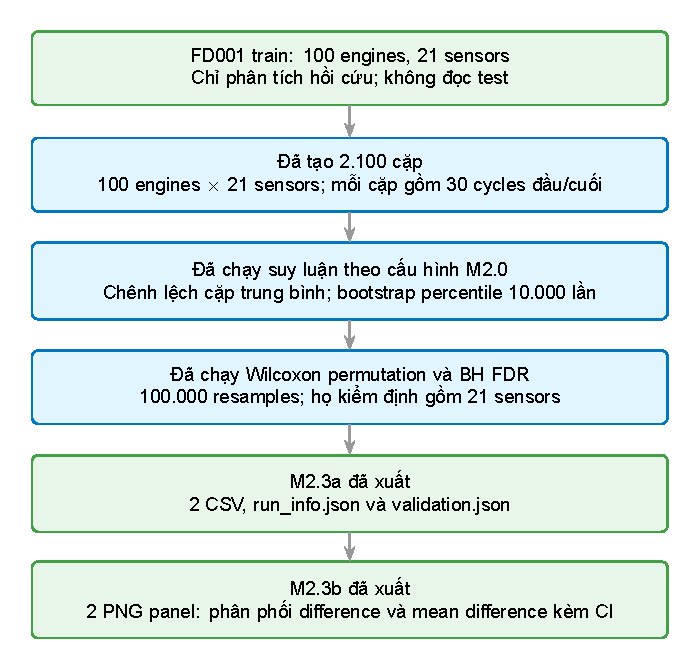
\includegraphics[width=0.91\linewidth]{figures/statistical-protocol.pdf}
\caption[Protocol thống kê đầu/cuối vòng đời]{Thiết kế phân tích mốc 2; chỉ bước chọn hai đoạn 30 cycles và các nguyên tắc đã nêu được chốt. Các phép tính suy luận chưa chạy, cấu hình chi tiết còn cần chốt.}
\label{fig:stat-protocol}
\end{figure}

\subsection{Đại lượng cần báo cáo và điều kiện diễn giải}
Bảng kết quả dự kiến giữ đủ 21 sensors, không chọn danh sách từ thứ hạng correlation của EDA. Ba operational settings không được gộp vào cùng họ giả thuyết sensor. Bảng cần có số cặp hợp lệ, số chênh lệch bằng 0, mức thay đổi, khoảng tin cậy, thống kê kiểm định, p-value gốc, p-value hiệu chỉnh và trạng thái có thể kiểm định.

Đề xuất dùng mean paired difference $\widehat\Delta_s=m^{-1}\sum_i D_{i,s}$ làm effect size theo đơn vị gốc, kèm median và phân phối $D_{i,s}$. Đây là đại lượng mô tả độ lớn thay đổi, không phải effect size chuẩn hóa và không so sánh trực tiếp độ lớn giữa các sensor khác thang đo. Không gán đơn vị vật lý nếu nguồn chưa xác nhận. Bootstrap lấy mẫu lại các engine cùng cặp $E,L$ để tạo khoảng tin cậy 95\% cho $\widehat\Delta_s$~\cite{scipyBootstrap}. Số lần lấy mẫu và phương pháp dựng khoảng còn ở mức đề xuất bên dưới.

Wilcoxon hai phía xét phân phối chênh lệch đối xứng quanh 0, với các cặp độc lập giữa engine~\cite{scipyWilcoxon}. Cần xem phân phối chênh lệch và ghi giới hạn đối xứng; bootstrap của mean không thay thế giả định này. Sensor hằng hoặc toàn bộ $D_{i,s}=0$ vẫn phải xuất hiện trong bảng dưới trạng thái không có biến thiên quan sát được. Không biến p-value không xác định thành 0 và không tự kết luận rằng sensor có giá trị dự đoán bằng 0.

Benjamini--Hochberg áp dụng cho một họ kiểm định đã xác định trước~\cite{benjamini1995fdr}. Đề xuất giữ họ gồm 21 sensors, dùng giá trị 1 chỉ trong vector hiệu chỉnh cho trường hợp không kiểm định được, đồng thời giữ p-value gốc là không áp dụng và ghi rõ trạng thái trong bảng. Quy ước này tránh thu nhỏ họ giả thuyết theo kết quả thuận lợi; nó không sửa được p-value thiếu hợp lệ hoặc bảo đảm FDR dưới mọi dạng phụ thuộc giữa sensors. Các khoảng tin cậy bootstrap riêng lẻ không phải simultaneous intervals.

\subsection{Cấu hình đề xuất cần chốt trước triển khai}
Các giá trị sau là đề xuất cụ thể để lượt triển khai có thể quyết định và ghi lại trước khi tính kết quả; chúng chưa phải cấu hình đã chạy hoặc quyết định do default thư viện tạo ra.
\begin{itemize}
\item Effect size chính: mean paired difference; kèm median để nhìn độ nhạy với phân phối lệch. Chưa bổ sung effect size chuẩn hóa nếu chưa có câu hỏi cần so sánh giữa sensors.
\item Bootstrap: 10.000 lần lấy mẫu lại 100 engines có hoàn lại, seed 42; đề xuất percentile interval tại các quantile 2,5\% và 97,5\%. Cần ghi rõ giới hạn độ bao phủ hữu hạn; không mặc định tương đương BCa. Trường hợp phân phối bootstrap suy biến phải gắn nhãn, không diễn giải khoảng bằng 0 là chắc chắn tuyệt đối.
\item Wilcoxon: hai phía; đề xuất bỏ zero differences theo quy ước \texttt{wilcox}, average ranks cho ties và phương pháp permutation khi cần xử lý ties/zeros. Số phép hoán vị và quy tắc làm tròn theo độ phân giải raw cần được cố định, kiểm tra bằng ví dụ tính tay trước khi chạy toàn bộ.
\item FDR: đề xuất $q=0{,}05$ trên họ 21 sensors như mô tả trên. Chưa tự thêm kiểm định thay thế hoặc điều chỉnh phương pháp dựa vào p-value vừa quan sát.
\end{itemize}

Phải chốt các mục còn mở này trước khi chạy mốc 2. Nếu dùng phương án khác, cập nhật protocol, lý do và thời điểm thay đổi trước khi tạo bảng kết quả; không trình bày lựa chọn mới như đã xác định từ đầu.

\subsection{Đầu ra và điều kiện nghiệm thu}
Đầu ra dự kiến gồm bảng cặp theo engine/sensor, bảng thống kê theo sensor, hình phân phối chênh lệch và effect size kèm khoảng tin cậy, cùng metadata ghi cấu hình và phiên bản. Không tạo artifact rỗng để thay kết quả chưa chạy.

Kiểm tra phải bao gồm chỉ số 30 cycles đúng trong từng engine, không chồng đoạn, ghép cặp một--một, ví dụ tính tay và trường hợp hằng/ties/zeros. Bootstrap phải lấy mẫu theo engine và giữ cặp; FDR cần được kiểm tra trên một vector p-value nhỏ có đáp án biết trước. Chạy lại với cùng input và seed phải tái lập kết quả; raw và EDA gốc giữ nguyên. Khi có kết quả mới cập nhật phần kết quả, nhật ký và bằng chứng kiểm tra.

Kết luận thống kê chỉ áp dụng cho thay đổi trên train mô phỏng theo protocol này. Phát hiện thay đổi không chứng minh quan hệ nhân quả hoặc hiệu quả dự đoán ngoài mẫu. Lựa chọn sensor cho mô hình vẫn phải học trong training fold; không dùng danh sách có ý nghĩa thống kê trên toàn train để chọn feature trước cross-validation.
